% -*- coding: utf-8 -*-
% !TEX TS-program = pdflatex
% !TEX encoding = UTF-8 Unicode

% Page Size (ISO A4)
\documentclass[a4paper,11pt,twoside]{book}
\pdfpagewidth 8.27in
\pdfpageheight 11.69in
\usepackage[total={8.27in,11.69in},]{geometry}
\geometry{inner=1in,outer=0.5in,top=0.5in,bottom=0.5in}
\geometry{bindingoffset=0.0in}

% Packages
\usepackage{graphicx}
\usepackage{sidecap}
\usepackage{booktabs} 
\usepackage{paralist} 
\usepackage{verbatim}
\usepackage[utf8]{inputenc}
\usepackage[T1]{fontenc}
\usepackage{subfig} 
\usepackage{xfrac} 
\usepackage[version=3]{mhchem} 
\usepackage[usenames,dvipsnames]{color}
\usepackage{hyperref} 
\hypersetup{ 
	pdftitle={Classic Macintosh Service Reference},
	pdfauthor={-}, 
	colorlinks=true, 		% ew, boxes 
	linkcolor=RoyalBlue, 		% internal links 
	citecolor=Violet, 		% bibliography 
	filecolor=Periwinkle, 		% external files 
	urlcolor=BlueViolet, 		% external links 
	}
\usepackage{float}
\usepackage{wrapfig}

% Section Title Appearance
\usepackage{sectsty}
\allsectionsfont{\fontfamily{ptm}\mdseries\upshape}
\sectionfont{\newpage\LARGE\centering\scshape}
\subsectionfont{\Large\scshape}
\subsubsectionfont{\large\bfseries}
\renewcommand{\sectionrule}{{\color{RoyalBlue}\rule[16pt]{\linewidth}{1.5pt}\vspace{-16pt}\\}}
\newcommand{\subsectionrule}{{\color{RoyalBlue}\rule[11pt]{\linewidth}{1pt}\vspace{-11pt}\\}}

% ToC (table of contents) Appearance
\usepackage[nottoc,notlof,notlot]{tocbibind} 
\usepackage[titles,subfigure]{tocloft} 
\renewcommand{\cftsecfont}{\Large\rmfamily\bfseries\upshape\color{CadetBlue}}
\renewcommand{\cftsecpagefont}{\rmfamily\mdseries\upshape} 

% Headers and Footers
\usepackage{fancyhdr} 
\pagestyle{fancy} 
\renewcommand{\headrulewidth}{0pt} 
\fancyhead{}
\fancyfoot{}
\fancyfoot[LE,RO]{\thepage}
\fancypagestyle{plain}{\fancyhf{}\fancyfoot[LE,RO]{\thepage}}

% Typeface Appearance
\renewcommand{\rmdefault}{ppl}
\renewcommand{\sfdefault}{jcl}
\renewcommand{\ttdefault}{pcr}

% !- Document STARTS HERE -!
\title{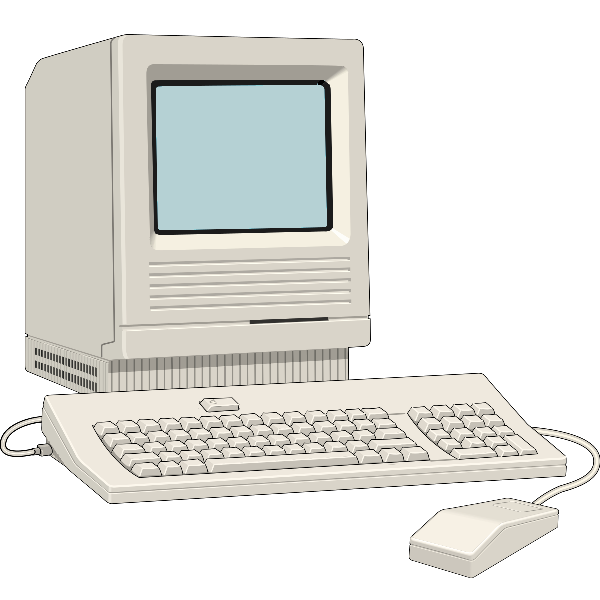
\includegraphics[height=4in]{toplevel/title.pdf} \\ ~ \\ ~ \\ \Huge{Classic Macintosh \\ Maintenance and Repair \\ } \huge{ ~ \\ \textsc{A Field Reference for Geeks}}}
\date{}
\author{Horst Burkhardt}

\begin{document}
\maketitle

\cleardoublepage
% -*- coding: utf-8 -*-

\chapter{Foreword}

\begin{center}
\textit{``Hello, I am Macintosh. It sure is great to get out of that bag!''}
\end{center}

\paragraph{%
On January the 24th of 1984, Macintosh introduced itself to the world. In comparison %
to the dolled-up computers we take for granted today, personal computers of the late %
1970s and early 1980s were ... rather impersonal. Personal meant that a person might %
own one, not that a person may be comfortable using one. Macintosh represented a fundamental %
shift in how people interacted with machines. \\
\textit{Instead of teaching humans about computers,} the theory went, %
\textit{we should teach computers about humans.} A laudable goal indeed, at a % 
time when most peoples' knowledge of computers was either arcade-style gaming or %
the necessity of memorising an arcane set of textual commands for getting work done. %
}

\begin{center}
\textit{``Unaccustomed as I am to public speaking, I'd like to share with you\\  a %
maxim I thought of the first time I met an IBM mainframe: \\Never trust a computer %
that you can't lift!''}
\end{center}

\paragraph{%
Macintosh was a computer for the masses. Every aspect of it was engineered to be %
appealing to the everyday user. Macintosh looked radically different from other %
personal computers of the time, many of which were shaped like suitcases or overly %
thick keyboards. Macintosh's price, too, was designed to be appealing - in comparison %
to the Lisa, with which it shared the 68000 at its heart and the idea of an entirely %
graphical interface, Macintosh was the very epitome of value, at \$2,495 (the Lisa cost %
\$9,995 at its inception, and at the time of Macintosh's introduction was still \$3,495 %
for a base model, a full thousand dollars more expensive than Macintosh.) %
}

\paragraph{%
Many books have been written about the historical context of Macintosh, and the line %
that dutifully followed it; hence, there is no need to go into greater detail here. %
This book exists to fulfill a need, and to fill a niche. There is a thriving community %
of people from many walks of life, from well-to-do collectors to impoverished students, %
united by a love of Macs. Unfortunately, many of the older Macs they so dearly love are %
rather past their prime; so much so that modular repairs are sometimes no longer sufficient %
to keep machines running. Component-level repair is becoming an unpleasant fact of life for %
those who would keep their Macintoshes in workable condition; among the prime culprits are %
aged capacitors and blown resistor networks. %
}

\paragraph{%
Of course, in repairing Macintoshes it helps to know something about them - how they should %
behave when working to specifications, and it especially helps to know what their limits and %
quirks are. For instance, while it is physically possible to install 32MB of RAM in a Colour %
Classic, no more than 10MB would be seen, and thus it would be a waste of (now fairly expensive) %
RAM SIMMs. %
}

\paragraph{%
This need is met, for users of Mac OS X and iOS, by a piece of software called Mactracker. It is also %
available for Windows, but has not been updated on that platform for some years. Formerly, it was %
available for Mac OS 8.6; this version has been withdrawn. A Linux port has been enquired about, %
and as of the time of writing, it has not materialised and is unlikely to. %
Ian Page has done a great good in making Mactracker available to the community at no %
charge, and it is a supremely useful resource which I recommend highly to anyone who works on Macs %
for their livelihood, or in their leisure. I would be lying to say that it has not been %
incredibly useful for researching the bulk of specifications in this tome. Thankfully %
I can get away with using the Windows version, outdated though it be, due to only covering %
Old World Macs. %
}

\paragraph{%
This book, however, seeks not only to provide the practical specifications of known Macintoshes, %
but also to collect, in one place, known repair techniques and background technical information. %
}

\cleardoublepage
% -*- coding: utf-8 -*-

\part{Specifications Database}

\chapter{Overview}

\paragraph{%
In knowing how to maintain any system, it is critical to know what the expected %
behaviour of that system is. Hence, this section of the book contains data on the %
stock configuration of all Old World Macintosh models (Performa-branded %
Macintoshes are not covered due to their being variations on a base model, %
a full listing will be present.) % 
}

\paragraph{%
This database is chiefly divided into two segments, for ease of navigation. The %
first, ``68k Macintoshes'', covers Macintoshes making use of the Motorola 68000 %
series microprocessors. These are identified by a lack of \textsl{\textbf{\textrm{PowerPC}}} %
branding on the case of the machine. The second segment, ``PowerPC Macintoshes'', %
covers Power Macintoshes and PowerBooks bearing the \textsl{\textbf{\textrm{PowerPC}}} logo; % 
these machines make use of a high-performance RISC CPU series principally designed by IBM. %
}

\paragraph{%
The data in the following pages is definitive, verified against multiple sources, including %
(where possible) the author's own collection. For machines not in the author's collection, %
data is provided based on at least two sources, three if possible, in order to minimise the %
risk of false information. The only disputable data is what constitutes the ``Optimal'' %
System Software version for a given Macintosh; this is based on the author's own %
experience and is entirely arbitrary. Caveat lector, your mileage may vary. %
}

\cleardoublepage
% -*- coding: utf-8 -*-

\chapter{68k Macintoshes}

\begin{center}
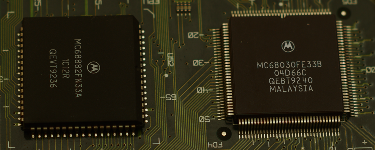
\includegraphics[height=1in]{68k/68030-68882-33.pdf} \\
\end{center}

\paragraph{\scriptsize{\textsc{%
68030 CPU and 68882 FPU from a Macintosh IIvx. This combination %
was used in many 68k Macintoshes to great effect. An FPU such as %
the one depicted here can improve performance in some applications %
by up to 80 percent.}}}

\paragraph{%
The Motorola 68000 series microprocessors were at the heart of every Macintosh %
until early 1994, when the first PowerPC-based workstations, known as Power %
Macintoshes, were released. Even after the release of the wildly successful %
Power Macintosh line, Macintoshes built around the 68040 were sold until %
their discontinuation in October of 1996. %
}

\paragraph{%
The Motorola 68000 microprocessor was, a full decade after its introduction to %
market, regarded widely as one of the most powerful and versatile production %
microprocessors available. It is worth noting that in this decade the %
significantly enhanced 68020 and 68030 had started to enjoy widespread use %
in workstations; no small praise then that the 68000 should stay relevant! %
}

\paragraph{%
On the topic of workstations, it is important to note a special machine which %
will not be covered in this text; the Macintosh XL. Ostensibly a repurposed %
Apple Lisa 2/10 with an Emulation Package allowing for the seamless execution %
of well-behaved Macintosh Software, the XL is not a Macintosh in the truest %
sense of the term; rather it is an inelegant attempt to recoup costs on a %
failed product. Aside from that attempting Lisa repairs or service in this %
day and age is an insane (not insanely great, merely insane) proposition, the %
Lisa falls outside the scope of this text. Information on the Lisa is, however, %
plentiful, if you know where to look, and I strongly encourage you to do so, if %
only to get a glimpse of what was a groundbreaking computer in its time. %
}

\paragraph{%
Several 68k microprocessors have been manufactured by Motorola over the years, %
and not all of them enjoy electrical similarities or code-compatibility. As such, %
it is important to note the particular microprocessors you will be dealing with. %
68000-series microprocessors likely to be found in the 68k Macintoshes you will %
come across are the 68000, 68020, 68030, 68LC040, and 68040. % 
}

% Compact Macs
% -*- coding: utf-8 -*-

\chapter{Compact Macs}

\input{68k/compact/mac128.tex}
\input{68k/compact/mac512.tex}
\input{68k/compact/macplus.tex}
\input{68k/compact/macse.tex}
\input{68k/compact/macse30.tex}
\input{68k/compact/classic.tex}
\input{68k/compact/classic2.tex}
\input{68k/compact/colourcl.tex}
\input{68k/compact/colourc2.tex}


% Macintosh II
% -*- coding: utf-8 -*-

\chapter{The Macintosh II}

\input{68k/macII/macII.tex}
\input{68k/macII/macIIx.tex}
\input{68k/macII/macIIcx.tex}
\input{68k/macII/macIIci.tex}
\input{68k/macII/macIIfx.tex}




\cleardoublepage
% -*- coding: utf-8 -*-

\chapter{PowerPC Macintoshes}

\paragraph{%
Introduced in Early 1994 with the x100 series Power Macintosh, the PowerPC was %
the beating heart of the Macintosh franchise until the middle of 2006, going %
through five generations of hardware made by Apple, and several other machines %
made by licenced Clone manufacturers such as UMAX, Radius, Daystar, and %
Motorola. While PowerPC-based machines did not completely displace their 68k %
forebears until October of 1996, with the discontinuation of the PowerBook 190cs, %
they quickly established themselves as Apple's mainstay. %
}

\paragraph{%
The transition from 68k to PowerPC was not without controversy, nor were the %
first-generation PowerPC machines without their foibles - in fact, it could be %
said that foibles and odd behaviours were a defining part of the Mac experience, %
if ever you had to spend a great deal of time working on Mac hardware or software%
... %
these foibles and unique Mac-only issues would continue well into the salad years %
of the Power Macintosh line. %
}

\paragraph{%
Here we concern ourselves only with the so-called ``Old World'' Power Macintoshes, %
that is to say any and all Power Macintoshes that look like Computers, as opposed %
to pieces of fruit. In practical terms, if you're looking for the specifics of a %
Power Macintosh G3 (Blue and White), another source is your best bet; but we'll %
be your faithful guide to anything up to and including the Power Macintosh G3 %
(tower), the ``Outrigger'' style Power Macintosh G3 (Desktop), and the infamous %
``Molar Mac'' Power Macintosh G3 (All-in-One). %
}


\end{document}